\documentclass[twocolumn,final]{svjour3}
\usepackage{graphicx}
\usepackage{hyperref}
\journalname{Software and Systems Modeling}
\begin{document}
\title{Guest editorial to the special section on ICMT at STAF 2018}
\author{Jesús Sánchez Cuadrado \and Arend Rensink}
\institute{
Jesús Sánchez Cuadrado \at Facultad de Informática, Universidad de Murcia, Campus de Espinardo, 30100 -- Murcia, Spain \\ \email{jesusc@um.es}
\and
Arend Rensink \at Department of Computer Science, University of Twente, P.O. Box 217, 7500 AE Enschede, Netherlands \\ \email{arend.rensink@utwente.nl}
}
\maketitle

\section{Introduction}

Modeling is a key element in reducing the complexity of software systems during their development and maintenance. Model transformations are essential for elevating models from documentation elements to first-class artifacts. Transformations also play a key role in analyzing models to reveal conceptual flaws or highlight quality bottlenecks and in integrating heterogeneous tools into unified tool chains.

Model transformation encompasses a variety of technical spaces, including modelware, grammarware, dataware, and ontoware, a variety of model representations, e.g., trees vs.\ graphs, and a variety of transformation paradigms including rule-based transformations, term re-writing, and manipulations of objects in general-purpose programming languages. Moreover, in other fields like compiler construction, the use of transformations is essential. Identifying means to reuse and share knowledge between fields is also of interest.

The study of model transformation includes foundations, structuring mechanisms, and properties, such as modularity and composability, transformation languages, techniques, and tools. An important goal of the field is the development of high-level model transformation languages, providing transformations that are amenable to higher-order model transformations or tailored to specific transformation problems. At the same time, usable and scalable verification techniques for model transformations are essential for the practical development of the field. The efficient execution of model queries and transformations by scalable transformation engines is also a key challenge. Novel algorithms as well as innovative (e.g., distributed) execution strategies and domain-specific optimizations are sought in this respect.

\section{This special section}

The \emph{International Conference on Model Transformation} (ICMT) is the premier forum for researchers and practitioners from all areas of model transformation. For many years now, it has been organised as part of \emph{Software Technologies: Applications and Foundations} (STAF), a federation of leading conferences on software technology. In this special section, we are proud to present extended versions of three of the best papers of ICMT 2018.

For the conference itself, all papers underwent rigorous peer reviewing by at least three experts, according to the high scientific standards set by STAF as well as Springer, resulting in an acceptance rate of roughly 35\%. Subsequently, for the special section, each paper was revised and extended, and subsequently received three more thorough reviews.

\medskip\noindent The three papers of this special section address a diverse cross-section of the topics of ICMT. We briefly discuss their contributions here.

\emph{Understanding {MDE} projects: megamodels to the rescue for architecture recovery} \cite{Understanding-MDE} presents an experience report on applying recovery to MDE projects. It is a necessary contribution for the MDE community to show how megamodels, architecture recovery and visualizations can work  together in order to help in understanding systems. The article shows that the accidental complexity of MDE (profusion of models, metamodels and transformations) can be addressed by MDE solutions; it also shows an original approach to MDE artifacts mining. 

\emph{{CoqTL}: A {Coq} {DSL} for Rule-Based Model Transformation} \cite{CoqTL} introduces a novel model transformation language called CoqTL, which
is implemented as an internal DSL in Gallina (the specification language of Coq). The goal of CoqTL is to facilitate proving transformation properties expressed as pre/postconditions, without having to translate the transformation into a different formal language. Thus, the paper brings Hoare-style verification to model transformation.

\emph{Comparing and Classifying Model Transformation Reuse Approaches across Metamodels} \cite{Transformation-Reuse} is a survey conducted by a large number of authors on the important topic of reuse, not of models but of model transformation. This paper is an important contribution to the MDE community, because of the fact that it give insight in the use of model transformations by (academic) practitioners, and it presents a thorough classification of various types of model transformation reuse. The combination of the survey and the classification is novel and gives a useful cross fertilisation. The results of the paper also show that there is still a long way to go to provide an easy access to all this to a practitioner.

\begin{acknowledgements}
We wish to thank the STAF organisational team in Toulouse for enabling us to organise the 2018 edition of the ICMT series, and the PC members for helping us to select the papers for the excellent programme. Furthermore, thanks to the SoSyM editor, Martin Schindler, for the support in organising this special section; and finally, the reviewers of the three papers presented here for their help in honing the papers to the best possible quality.
\end{acknowledgements}


\nocite{*}
\bibliographystyle{spmpsci}
\bibliography{editorial}

\noindent \textbf{Jesús Sánchez Cuadrado} did lots of cool stuff.

\medskip\noindent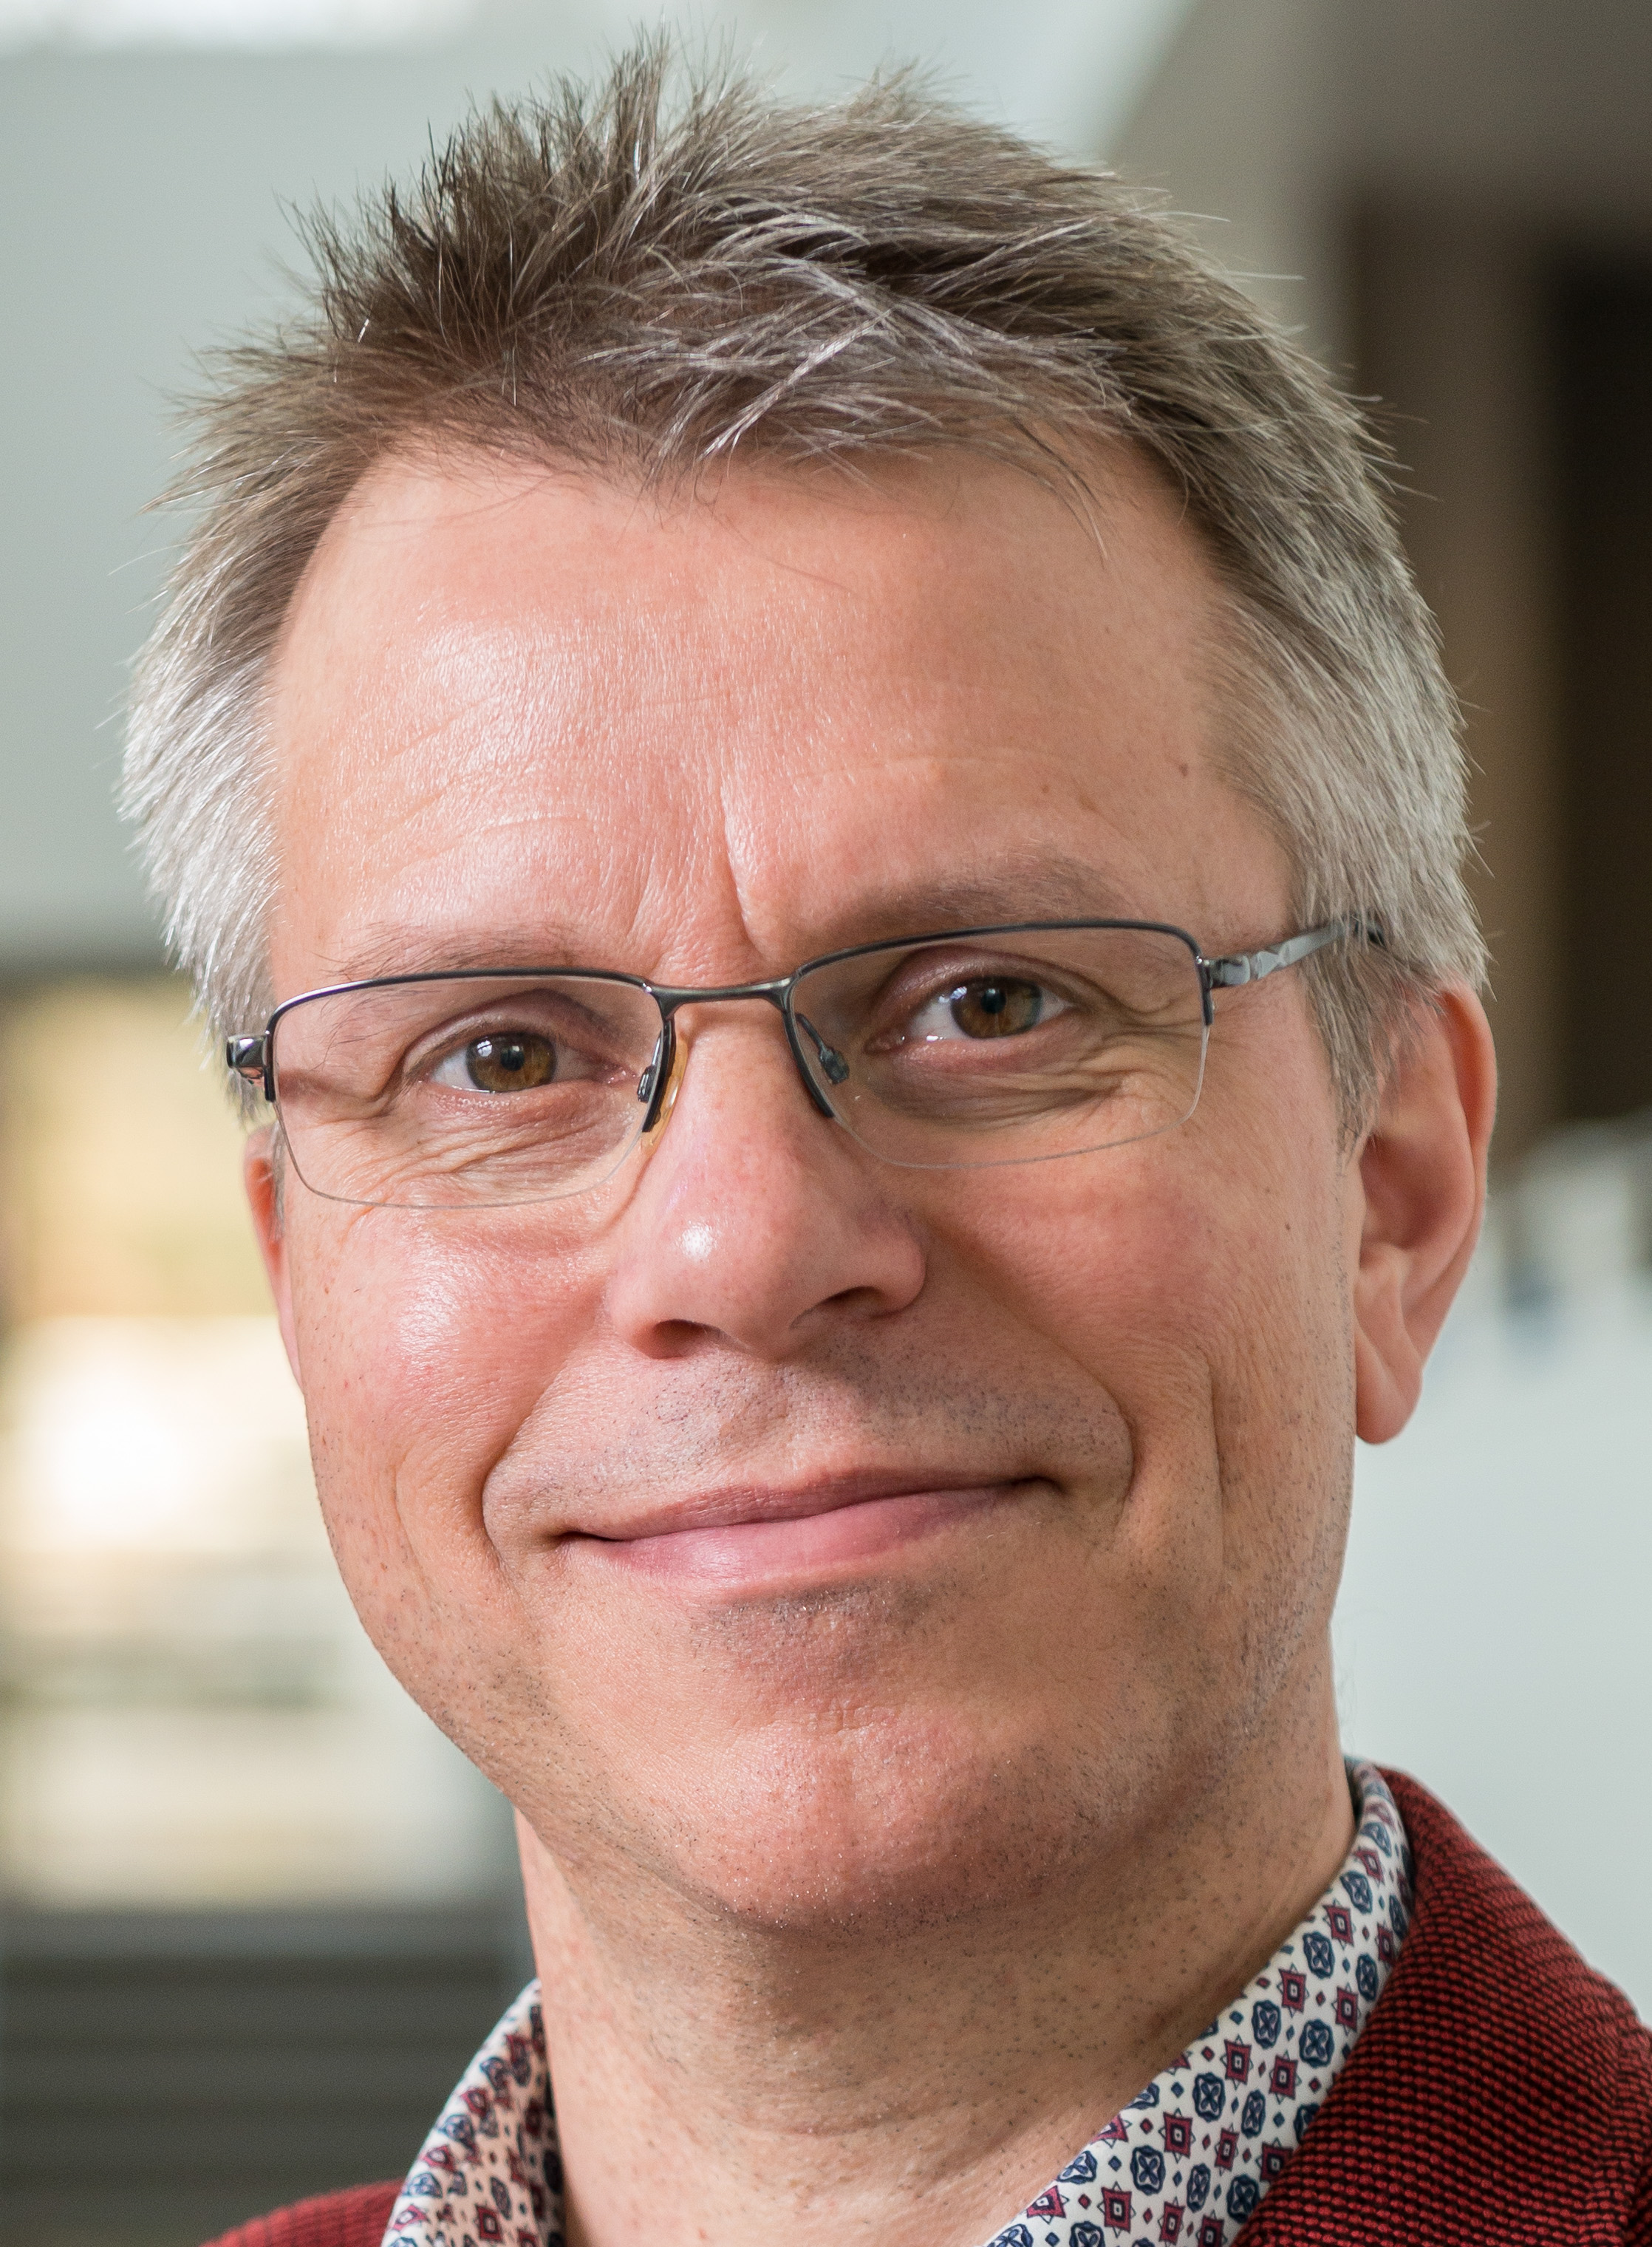
\includegraphics[width=.2\textwidth]{arend}
\noindent \textbf{Arend Rensink} received his PhD degree in 1993. His research interests range from process algebra (in particular action refinement), graph and model transformation and verification to software maintainability in general. He is the creator of the award-winning graph transformation tool \href{https://sf.net/projects/groove}{GROOVE}. Since 2011 he has held the chair on \emph{Software Modelling, Transformation and Verification} at the University of Twente, and since 2018 he is also Programme Director of the Computer Science Bachelor and Master programmes.

\end{document}



%%% Local Variables:
%%% mode: latex
%%% TeX-master: t
%%% End:
